\section{Predication}
\label{sec:predication}

For the reasons outlined in section \ref{sec:costo_of_branch_prediction}, we can conclude that branches are expensive. Even when using state-of-the-art branch predictors, certain branches are systematically hard to predict or have such low occurrences that not enough data are collected to perform a good prediction \cite{lin2019branch}.
Predication is used to replace conditional branches with other instructions. In \textit{LLVM} and in \textit{GCC}, this is usually done during the backend optimization phase where the compiler works on the machine-level representation of the code. The name that is generally given to this code optimization pass is \texttt{if-conversion}.

\begin{figure}[h!]
\centering
\begin{tabular}{ c c c }
\adjustbox{valign=m}{%
\begin{lstlisting}[language=C++, basicstyle=\ttfamily\small]
if (x > 0) y = 10;
else       y = 20;
\end{lstlisting}
}
&
\begin{tikzpicture}
    \draw[->, line width=0.5pt] (0,0) -- (1.5,0);
\end{tikzpicture}
&
\adjustbox{valign=m}{%
\begin{lstlisting}[language=C++, basicstyle=\ttfamily\small]
y = (x > 0)  * 10 + 
    (x <= 0) * 20;
\end{lstlisting}
}
\end{tabular}
\caption[Replacing a Conditional Branch with Arithmetic Operations]{Replacing a conditional branch with arithmetic operations.}
\label{fig:branching_predication_example}
\end{figure}

An example of this is presented in figure \ref{fig:branching_predication_example} where code containing a conditional branch is replaced with code that performs exactly the same operation without the use of conditional branches. The example presented uses arithmetic properties to replace the branch and is usually referred to as \textit{Arithmetic Predication} or \textit{Branchless Programming}. Using Arithmetic Predication to replace branches presents limitations: multiplications are also expensive, and it is difficult to apply most of the time.

One way to overcome these limitations is by utilizing predicated instructions supported by the architecture when these are available. A predicated instruction in \armvs is an instruction that attaches conditions directly to instructions, allowing them to either execute or skip based on the condition's outcome. \newline

\noindent\begin{minipage}{.45\textwidth}
\begin{lstlisting}[caption=Standard MOV in ARMv7 assembly, style=AsmStyle, label={lst:add}]{Name}
MOV R0, R1
\end{lstlisting}
\end{minipage}\hfill
\begin{minipage}{.45\textwidth}
\begin{lstlisting}[caption=Predicated MOV in ARMv7 assembly, style=AsmStyle, label={lst:cadd}]{Name}
MOVGT R0, R1
\end{lstlisting}
\end{minipage}

The \armvs architecture supports several predicated instructions. For example, the standard \texttt{MOV} instructions in listing \ref{lst:add} takes the value in \texttt{R1} and moves it into \texttt{R0} while, the predicated version, \texttt{MOVGT}, showed in listing \ref{lst:cadd} moves the value in \texttt{R1} to \texttt{R0} only when the last comparison was "greater than". \\

\begin{figure}[h!]
\centering
\begin{tabular}{ c c c c }
\adjustbox{valign=m}{%
\begin{lstlisting}[language=C++, basicstyle=\ttfamily\small]
if (x > 0) y = 10;
else y = 20;
\end{lstlisting}
}
&
\adjustbox{valign=m}{%
\begin{tikzpicture}
    \draw[->, line width=0.5pt] (0,0.5) -- (2, 1.5);
    \draw[->, line width=0.5pt] (0,-0.5) -- (2, -1.5);
\end{tikzpicture}
}
&
\adjustbox{valign=m}{%
\begin{minipage}{0.4\textwidth}
\textbf{Without Predication:}
\begin{lstlisting}[basicstyle=\ttfamily\small]
    cmp r0, #0
    bgt greater
    mov r1, #20
    b end
greater:
    mov r1, #10
end:
\end{lstlisting}

\vspace{0.8cm} % Space between the two assembly listings

\textbf{With Predication:}
\begin{lstlisting}[basicstyle=\ttfamily\small]
    cmp r0, #0
    movgt r1, #10
    movle r1, #20
\end{lstlisting}
\end{minipage}
}
\end{tabular}
\caption{Branching versus predication in \texttt{ARM} assembly}
\label{fig:branching_predication_ARM}
\end{figure}

In figure \ref{fig:branching_predication_ARM} two assembly translations of the code in Figure \ref{fig:branching_predication_example} are displayed. The top one is when no predication is used, while the bottom one uses predicated instructions.
By comparing the two versions in Figure \ref{fig:branching_predication_ARM}, the benefits of predication are staggering. The code size is reduced from five instructions to three while removing one conditional branch and one unconditional branch. Another benefit that is outlined by this example is \textit{Deterministic Execution}. It's difficult to predict how many cycles an assembly code needs to be executed when branch predictions and other forms of speculations are involved. As we removed all the branches and as we have no memory accesses in our snippet of code, we can determine exactly how long it's going to take to execute the operation. Deterministic Execution is crucial in certain fields where the software needs to have predictable behavior and respond within strict timing constraints. This is necessary for instance in flight control systems, medical devices, and other mission-critical software.
Section \ref{sec:arch_support} focuses on a more in-depth analysis of how \armvs and \texttt{IA64} architectures introduce support for predication. It is also necessary to mention some limitations of predication.
\begin{itemize}
    \item \textit{Increased Instruction Executions}: Predication can lead to unnecessary execution of both paths in a conditional statement. In certain cases, this may lead to a very inefficient use of the CPU and to wasting several cycles. This is particularly true when the predicated code has long conditional chains.
    \item \textit{Higher register pressure}: As we might need to hold intermediate results in registers, the register pressure increases. Registers are a highly contented resource, and allocating them efficiently is a difficult problem in compilers \cite{chaitin1981register}. If the increased pressure introduced by predication results in spilling to memory, performance degradation is to be expected.
    \item \textit{Code Size}: While the example presented,  demonstrates how predication can result in code size reduction, this is not necessarily the case. In fact, as a more complex control flow is taken into account, code size is more likely to increment.
\end{itemize}

For these reasons, if predication is applied indiscriminately, performance regression happens. Production compilers like \textit{LLVM} and \textit{GCC} use heuristics to decide at compile time whether predication is beneficial or not. In subsection \ref{sec:compiler_heuristics} we will treat this in more detail reporting and analyzing some of these heuristics. Finding whether predication is applicable is per se a challenge. The logic that \textit{LLVM} uses to find basic blocks where predication is applicable is reported in subsection \ref{sec:detecting_pred} while Subsection \ref{sec:limitations} talks about compilers' limitation and shows an example where \textit{LLVM} fails to identify \textit{if-conversion}. Lastly, in subsection \ref{sec:predication_benchmark}, a series of micro-benchmarks will be proposed to showcase in which cases and what impact \textit{if-conversion} has.

\subsection{How is Predication Achieved in the Architecture}
\label{sec:arch_support}
Various ways to support predication at the ISA level have been developed. In the case of \armvs, predication is achieved through condition flags in the \textit{Program Status Register} (PSR) and the instruction’s condition field,
This is a special register used to set various bits that describe the execution state, among these bits, there are the Zero (Z), Negative (N), Carry (C), and Overflow (V) bits which are set whenever an arithmetic instruction is executed.
When the CPU encounters a predicated instruction, it evaluates the condition field against the current PSR flags. If the condition is met, the instruction executes; otherwise, it is treated as a no-op.

\begin{figure}[H]
    \centering
    \begin{center}
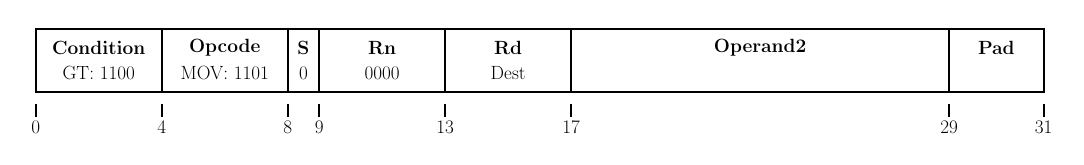
\begin{tikzpicture}[scale=0.4, every node/.style={scale=0.4}]
    % Bit fields with adjusted widths and labels for clarity
    \draw[thick] (0,0) rectangle (4,2) node[midway, yshift=0.4cm] {\textbf{\LARGE Condition}};
    \node at (2, 0.6) {\LARGE GT: 1100};
    
    \draw[thick] (4,0) rectangle (8,2) node[midway, yshift=0.4cm] {\textbf{\LARGE Opcode}};
    \node at (6, 0.6) {\LARGE MOV: 1101};
    
    \draw[thick] (8,0) rectangle (9,2) node[midway, yshift=0.4cm] {\textbf{\LARGE S}};
    \node at (8.5, 0.6) {\LARGE 0};
    
    \draw[thick] (9,0) rectangle (13,2) node[midway, yshift=0.4cm] {\textbf{\LARGE Rn}};
    \node at (11, 0.6) {\LARGE 0000};
    
    \draw[thick] (13,0) rectangle (17,2) node[midway, yshift=0.4cm] {\textbf{\LARGE Rd}};
    \node at (15, 0.6) {\LARGE Dest};
    
    \draw[thick] (17,0) rectangle (29,2) node[midway, yshift=0.4cm] {\textbf{\LARGE Operand2}};
    
    \draw[thick] (29,0) rectangle (32,2) node[midway, yshift=0.4cm] {\textbf{\LARGE Pad}};
    
    % Bit numbers
    \draw[thick] (0,-0.4) -- (0,-0.8) node[below] {\LARGE 0};
    \draw[thick] (4,-0.4) -- (4,-0.8) node[below] {\LARGE 4};
    \draw[thick] (8,-0.4) -- (8,-0.8) node[below] {\LARGE 8};
    \draw[thick] (9,-0.4) -- (9,-0.8) node[below] {\LARGE 9};
    \draw[thick] (13,-0.4) -- (13,-0.8) node[below] {\LARGE 13};
    \draw[thick] (17,-0.4) -- (17,-0.8) node[below] {\LARGE 17};
    \draw[thick] (29,-0.4) -- (29,-0.8) node[below] {\LARGE 29};
    \draw[thick] (32,-0.4) -- (32,-0.8) node[below] {\LARGE 31};

\end{tikzpicture}
\end{center}
    \begin{center}
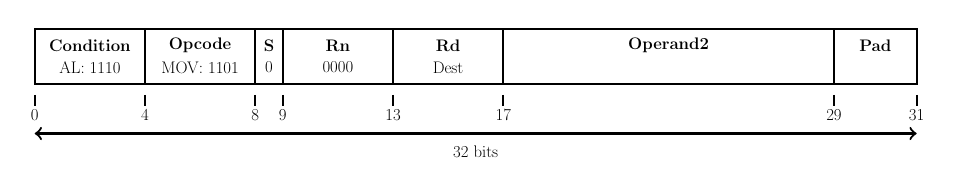
\begin{tikzpicture}[scale=0.35, every node/.style={scale=0.35}]
    % Bit fields with adjusted widths and labels for clarity
    \draw[thick] (0,0) rectangle (4,2) node[midway, yshift=0.4cm] {\textbf{\LARGE Condition}};
    \node at (2, 0.6) {\LARGE AL: 1110};
    
    \draw[thick] (4,0) rectangle (8,2) node[midway, yshift=0.4cm] {\textbf{\LARGE Opcode}};
    \node at (6, 0.6) {\LARGE MOV: 1101};
    
    \draw[thick] (8,0) rectangle (9,2) node[midway, yshift=0.4cm] {\textbf{\LARGE S}};
    \node at (8.5, 0.6) {\LARGE 0};
    
    \draw[thick] (9,0) rectangle (13,2) node[midway, yshift=0.4cm] {\textbf{\LARGE Rn}};
    \node at (11, 0.6) {\LARGE 0000};
    
    \draw[thick] (13,0) rectangle (17,2) node[midway, yshift=0.4cm] {\textbf{\LARGE Rd}};
    \node at (15, 0.6) {\LARGE Dest};
    
    \draw[thick] (17,0) rectangle (29,2) node[midway, yshift=0.4cm] {\textbf{\LARGE Operand2}};
    
    \draw[thick] (29,0) rectangle (32,2) node[midway, yshift=0.4cm] {\textbf{\LARGE Pad}};
    
    % Bit numbers
    \draw[thick] (0,-0.4) -- (0,-0.8) node[below] {\LARGE 0};
    \draw[thick] (4,-0.4) -- (4,-0.8) node[below] {\LARGE 4};
    \draw[thick] (8,-0.4) -- (8,-0.8) node[below] {\LARGE 8};
    \draw[thick] (9,-0.4) -- (9,-0.8) node[below] {\LARGE 9};
    \draw[thick] (13,-0.4) -- (13,-0.8) node[below] {\LARGE 13};
    \draw[thick] (17,-0.4) -- (17,-0.8) node[below] {\LARGE 17};
    \draw[thick] (29,-0.4) -- (29,-0.8) node[below] {\LARGE 29};
    \draw[thick] (32,-0.4) -- (32,-0.8) node[below] {\LARGE 31};

    % Arrow for full bit length label
    \draw[<->, thick] (0,-1.8) -- (32,-1.8) node[midway, below, yshift=-0.3cm] {\LARGE 32 bits};
\end{tikzpicture}
\end{center}

    \caption[\texttt{ARMv7}'s Bit-level Encoding]{Bit-level encoding of \texttt{ARMv7}'s \texttt{MOVGT} (on top) and of \texttt{MOV} (on the bottom) instructions, illustrating fields for condition codes, opcode, status bit, register operands, and operand values.}
    \label{fig:mov_encoding}
\end{figure}

In figure \ref{fig:mov_encoding} we can observe how \texttt{MOV} and \texttt{MOVG} bit encoding only differ for the first four bits. The condition field in \armvs applies to almost all instructions. In ARM's architecture, most instructions have a 4-bit condition field. This makes non-predicated instructions a particular case of predication where the condition field is set to \texttt{1110}. \\

Another architecture design that offers predication support is the Itanium \texttt{IA-64}.
The \texttt{IA-64} has 64 predicate registers (\texttt{p0} to \texttt{63}) that allow each instruction to be conditionally executed based on specific predicate values. Each instruction can specify a predicate register, offering highly granular control over conditional execution. Using this, approach, entire sections of code can be totally predicated, minimizing the dependency on branch predictors.

\begin{center}
\begin{minipage}{0.5\textwidth}
\begin{lstlisting}[caption=Predicated MOV in Itanium,frame=tlrb,label={lst:itanium_predicated}]
cmp.gt p1, p0 = r0, #0
(p1) mov r1 = 10
(p0) mov r1 = 20
\end{lstlisting}
\end{minipage}
\end{center}

In listing~\ref{lst:itanium_predicated}, it is possible to see the \texttt{IA-64} equivalent of the assembly code showed in listing \ref{fig:branching_predication_ARM}.

It is important to mention that no modern \textit{ISA} has a predication support that is as central as \texttt{ARMv7}. If we look at \texttt{x86}, \texttt{RISC-V} and even the more recent version of \texttt{ARM} such as \texttt{ARMv8} and \texttt{ARMv9}, none of them decided to give predication such a central role.
This may prove that there are better architectural choices that grant higher performances than such extensive predication support.
In the specific case of \texttt{ARM}, the direction that has been taken is towards a more lean architecture with less complex instructions. This allows for a design that is smaller in terms of area and allows using the encoding space that was before used by the predication to double the number of available registers \cite{armv8_instruction_removal}. 
Nevertheless, all the modern \textit{ISA} surveyed still present support for a small set of predicated instructions.

\subsection{Detecting Predicable Regions}
\label{sec:detecting_pred}

Some operations are difficult to predicate. Interruption, Exceptions, and System Calls have side effects that expand beyond the local execution and might trigger events that are impossible to revert. Certain Control Flow Instructions like \texttt{jmp} and \texttt{call} alter the program's execution path, predicating this requires hardware to simulate both the taken and non-taken paths simultaneously.
Additionally, predicating large blocks results in executing many unnecessary instructions when the predicate is false. The performance penalty of executing unnecessary instructions outweighs the benefit of avoiding a branch. A set of basic block is therefore considered not predicable if it exceeds certain sizes.

The discovery of predicable regions is the beginning of the \texttt{if-conversion} step. This optimization pass starts by iterating through all the basic blocks in a function's control flow graph (CFG).

\begin{figure}[H]
    \centering
    \begin{lstlisting}[style=CStyle]
/// Analyze the structure of the sub-CFG starting from the specified block.
/// Record its successors and whether it looks like an if-conversion candidate.
void IfConverter::AnalyzeBlock(
    MachineBasicBlock &MBB, std::vector<std::unique_ptr<IfcvtToken>> &Tokens) {
  // Initialize stack with the starting block.
  SmallVector<MachineBasicBlock *, 16> BBStack = {&MBB};

  while (!BBStack.empty()) {
    MachineBasicBlock *BB = BBStack.pop_back_val();
    BBInfo &BBI = BBAnalysis[BB->getNumber()];

    // Skip blocks already analyzed.
    if (BBI.IsAnalyzed) 
      continue;

    // Analyze branches and instructions in the block.
    AnalyzeBranches(BBI);
    ScanInstructions(BBI, BB->begin(), BB->end());

    // Skip blocks unsuitable for if-conversion.
    if (!BBI.IsBrAnalyzable || BBI.BrCond.empty()) {
      BBI.IsAnalyzed = true;
      continue;
    }

    // Push successors for further analysis.
    if (BBI.TrueBB && BBI.FalseBB) {
      BBStack.push_back(BBI.TrueBB);
      BBStack.push_back(BBI.FalseBB);
    }

    // Check for if-conversion patterns (e.g., diamonds, triangles).
    if (ValidDiamond(BBI)) {
      Tokens.push_back(std::make_unique<IfcvtToken>(BBI, ICDiamond));
    } else if (ValidTriangle(BBI)) {
      Tokens.push_back(std::make_unique<IfcvtToken>(BBI, ICTriangle));
    } else if (ValidSimple(BBI)) {
      Tokens.push_back(std::make_unique<IfcvtToken>(BBI, ICSimple));
    }

    BBI.IsAnalyzed = true;
  }
}
\end{lstlisting}
    \caption[\texttt{AnalyzeBlock} Implementation for \texttt{ARM} Architectures]{Simplified version of \textit{LLVM}'s \texttt{AnalyzeBlock} implementation for \texttt{ARM} architectures.}
    \label{fig:analyze_block}
\end{figure}

For each block, the function \texttt{AnalyzeBlock} is called. A simplified version of this function is shown in Listing \ref{fig:analyze_block}.

A \textit{MachineBasicBlock} is a basic block after being translated to machine instructions.
This function analyzes the structure of a \texttt{sub-CFG} starting from a given \texttt{MachineBasicBlock}. It evaluates branches and records successors to determine if the block is suitable for \texttt{if-conversion}.
The function \texttt{AnalyzeBranches}, determines if its branches can be analyzed or reversed, and checks if it has fall-through behavior. The data collected when this function runs are then stored in the \texttt{MachineBasicBlock} struct and used later. The function \texttt{ScanInstruction} scans all the instructions in the block to determine if the block is predicable. In most cases, a block is predicable if all the instructions in the block are predicable.
If the sub-CFG is not predicable, no further analysis are performed. If it is, certain patterns are searched in the sub-CFG graph. \\

\begin{figure}[H]
    \centering
    \begin{minipage}{0.45\textwidth}
  % Code Listing
  \begin{lstlisting}[style=Cstyle]
void triangleBranch(int condition) {
    // EBB: Entry Basic Block
    x_ ++;
    if (x == 0) {
        // TBB: True Block
        x_ = 42;
    }
    // FBB: Fall-through Block
    y_ = 100; // Common operation
}
  \end{lstlisting}
  \end{minipage}%
  \hfill
  \begin{minipage}{0.5\textwidth}
  \centering
  % Triangle Branch Diagram
  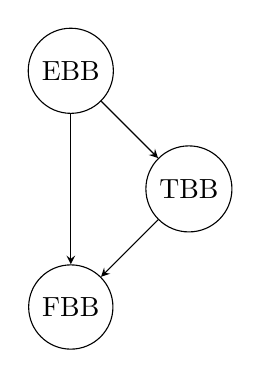
\begin{tikzpicture}[node distance=1.5cm and 2cm, >=stealth]
      % Nodes
      \node[circle, draw, fill=white, minimum size=0.8cm] (EBB) at (0, 3) {EBB};
      \node[circle, draw, fill=white, minimum size=0.8cm] (TBB) at (1.5, 1.5) {TBB};
      \node[circle, draw, fill=white, minimum size=0.8cm] (FBB) at (0, 0) {FBB};

      % Edges
      \draw[->] (EBB) -- (TBB);
      \draw[->] (EBB) -- (FBB);
      \draw[->] (TBB) -- (FBB);
  \end{tikzpicture}
  \end{minipage}

    \caption[TBB and fall through FBB]{The C++ code on the left, has a EBB, a TBB and a fall through FBB. When compiled it gives origin to the triangular branch on the right.}
    \label{fig:triangle_branch}
\end{figure}

The most simple pattern identified in the CFG is a \textit{Triangular Branch}, an example is shown in Figure \ref{fig:triangle_branch}. This control flow pattern begins with an \textit{Entry Basic Block} (EBB) which branches into a \textit{True Basic Block} (TBB). Both the EBB and TBB subsequently converge into the \textit{False Basic Block} (FBB).

When a \textit{Triangular Branch} is identified when using \textit{ARMv7} as the target architecture, given the analysis already performed and the hardware support, we know that it can be predicated. The last step is therefore to verify if the number of instructions to be predicated is within the limit. This is performed in the function \texttt{MeetIfcvtSizeLimit}. The logic used in this function to calculate the number of instruction is reported in Listing \ref{fig:predication_size}.

\begin{figure}[H]
    \centering
    \begin{lstlisting}[style=CStyle]
unsigned NumPredicatedInstructions = 0;

// Count instructions to be predicated in the true block
for (auto &I : make_range(TIB, TIE)) {  // TIB and TIE mark the range
    NumPredicatedInstructions++;
}

// Count instructions to be predicated in the false block
for (auto &I : make_range(FIB, FIE)) {  // FIB and FIE mark the range
    NumPredicatedInstructions++;
}

if (NumPredicatedInstructions > 15)
  // Do not predicate
\end{lstlisting}
    \caption{Logic used in \textit{LLVM} to decide if a block is too big to be predicated.}
    \label{fig:predication_size}
\end{figure}

The number of instructions to be predicated is determined by counting the number of instructions in the TIB and in the FIB. Each instruction in these ranges is counted, incrementing the \texttt{NumPredicatedInstructions} variable. If the total number of predicated instructions exceeds a predefined threshold of 15, the function decides not to proceed with predication, ensuring that excessively large predicated blocks are avoided to maintain efficiency.

In the case of the \textit{Triangular Branch}, the FIB is common to both branches, therefore the size only depends on the number of instructions in the TIB. In figure \ref{fig:triangle_asm}, the before and after in machine code is shown for the code provided in figure \ref{fig:triangle_branch}

\begin{figure}[H]
    \centering
    \begin{center}
    % First Assembly and CFG
    \begin{minipage}{0.22\textwidth}
    \begin{lstlisting}[style=AsmStyle]
triangleBranch:
  LDR R0, =x_
  LDR R1, [R0]
  ADD R1, R1, #1
  STR R1, [R0]
  CMP R1, #0
  BEQ FBB
  LDR R0, =x_
  MOV R1, #42
  STR R1, [R0]
FBB:
  LDR R0, =y_
  MOV R1, #100
  STR R1, [R0]
  BX LR
    \end{lstlisting}
    \end{minipage}
    \hfill
    \begin{minipage}{0.22\textwidth}
    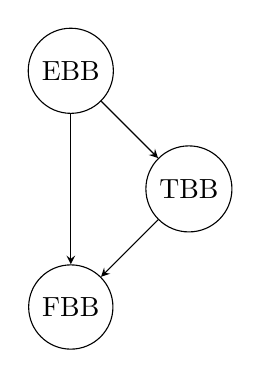
\begin{tikzpicture}[node distance=1.5cm and 2cm, >=stealth]
        \node[circle, draw, fill=white, minimum size=0.8cm] (EBB) at (0, 3) {EBB};
        \node[circle, draw, fill=white, minimum size=0.8cm] (TBB) at (1.5, 1.5) {TBB};
        \node[circle, draw, fill=white, minimum size=0.8cm] (FBB) at (0, 0) {FBB};

        \draw[->] (EBB) -- (TBB);
        \draw[->] (EBB) -- (FBB);
        \draw[->] (TBB) -- (FBB);
    \end{tikzpicture}
    \end{minipage}
    \hfill
    % Second Assembly and CFG
    \begin{minipage}{0.22\textwidth}
    \begin{lstlisting}[style=AsmStyle]
triangleBranch:
  LDR R0, =x_
  LDR R1, [R0]
  ADD R1, R1, #1
  STR R1, [R0]
  CMP R1, #0
  @@MOV R3, #42
  @MOV R4, #100
  @@IT NE
  @@MOVNE R1, R3
  @@MOVEQ R1, R4
  STR R1, [R0]
  LDR R0, =y_
  STR R4, [R0]
  BX LR
    \end{lstlisting}
    \end{minipage}
    \hfill
    \begin{minipage}{0.22\textwidth}
    
\begin{tikzpicture}[node distance=1.5cm and 2cm, >=stealth]
        \node[circle, draw, fill=white, minimum size=0.8cm] (EBB) at (0, 3) {EBB};
    \end{tikzpicture}
    \end{minipage}
    \end{center}
    \caption[TriangleBranch Comparison]{Comparison of assembly code and control flow graphs (CFGs) for \texttt{triangleBranch}: original code with branching versus optimized code with predication, demonstrating CFG simplification.}
    \label{fig:triangle_asm}
\end{figure}


Three other patterns exist: \textit{Diamond}, \textit{Forked Diamond} and \textit{Simple}. Each of these patterns requires a different size and feasibility analysis to determine if they can be \textit{if-converted}.

\subsection{Compiler's Heuristics}
\label{sec:compiler_heuristics}

As demonstrated in section \ref{sec:predication} and highlighted by August et al. \cite{August98}, indiscriminate use of predication leads to performance degradation.
To determine whether to apply this technique, modern compilers rely on heuristics. The heuristics are highly architecture-dependent, as illustrated in Table \ref{tab:misprediction_penalty}. In the rest of this section, the heuristics used by the production state-of-the-art compiler \textit{LLVM} is described.

Section \ref{sec:detecting_pred} already introduced that, when analyzing a block for \textit{if-conversion} the possible cost is computed. The cost of predicating a Basic Block consists of two components: architecture-dependent predication cost and instruction latency. These costs vary based on the specific instruction and the architecture. Some architectures impose a fixed cost for predicating any instruction, while others either avoid this cost entirely or apply it selectively to certain instructions. Importantly, the cost of predication associated with each instruction is not arbitrarily defined by the compiler but instead reflects the actual cost of executing the instruction on the target architecture. Taking as reference the \texttt{ARMv7} architecture, calls have an additional latency of 1 cycle to be predicated, while predicating any other instruction does not introduce any additional cost. It's important to note that compared to other architectures, predication in \texttt{ARMv7} is a central part of the architecture and therefore using it does not present relevant overheads.

\begin{figure}[H]
    \centering
    \begin{lstlisting}[style=CStyle]
BBI.NonPredSize++;
unsigned ExtraPredCost = TII->getPredicationCost(MI);
unsigned NumCycles = SchedModel.computeInstrLatency(&MI, false);
if (NumCycles > 1)
    BBI.ExtraCost += NumCycles-1;
BBI.ExtraCost2 += ExtraPredCost;
\end{lstlisting}
    \caption[Predication Cost Calculation]{Portion of code where the cost of predicating a Basic Block is calculated in \textit{LLVM}.}
    \label{lst:predication_cost}
\end{figure}

The impact of predication can be both positive and negative on the number of cycles needed to execute a function. When the cost is negative, we always choose to apply the \textit{if-conversion} transformation. On the other hand, having a positive cost does not automatically rule out predication. Instead, we apply a further heuristic that takes into account the cost of misprediction.
The logic to perform the cost analysis of predication is in the function \texttt{ScanInstruction} which is partially reported in listing \ref{lst:predication_cost}

\begin{figure}[H]
    \centering
    \begin{lstlisting}[style=CStyle]
bool ARMBaseInstrInfo::
isProfitableToIfCvt(MachineBasicBlock &TBB,
                    unsigned TCycles, unsigned TExtra,
                    MachineBasicBlock &FBB,
                    unsigned FCycles, unsigned FExtra,
                    BranchProbability Probability) const {
  if (!TCycles)
    return false;

  // Attempt to estimate the relative costs of predication versus branching.
  // Here we scale up each component of UnpredCost to avoid precision issue when
  // scaling TCycles/FCycles by Probability.
  const unsigned ScalingUpFactor = 1024;

  unsigned PredCost = (TCycles + FCycles + TExtra + FExtra) * ScalingUpFactor;
  unsigned UnpredCost;
  if (!Subtarget.hasBranchPredictor()) {
    // This code block contains the case where a pranch predictor
    // is not available. For the sake of brevity is not reported
  } else {
    unsigned TUnpredCost = Probability.scale(TCycles * ScalingUpFactor);
    unsigned FUnpredCost =
      Probability.getCompl().scale(FCycles * ScalingUpFactor);
    UnpredCost = TUnpredCost + FUnpredCost;
    UnpredCost += 1 * ScalingUpFactor; // The branch itself
    UnpredCost += Subtarget.getMispredictionPenalty() * ScalingUpFactor / 10;
  }

  return PredCost <= UnpredCost;
}
\end{lstlisting}
    \caption{\textit{LLVM}'s \texttt{isProfitableToIfCvt} implementation for \texttt{ARM} architectures.}
    \label{lst:predications_heuristic}
\end{figure}

The cost used in \texttt{isProfitableToIfCvt} are:

\begin{itemize}
    \item \textbf{TCycles}: The execution time (in cycles) of the "True" block.
    \item \textbf{TExtra}: Additional cost (in cycles) for predicating the "True" block.
    \item \textbf{FCycles}: The execution cost (in cycles) of the "False" block.
    \item \textbf{FExtra}: Additional cost (in cycles) for predicating the "False" block.
\end{itemize}

The actual cost of predication is calculated on line 15 of listing \ref{lst:predications_heuristic}:
\[
\text{PredCost} = (\text{TCycles} + \text{FCycles} + \text{TExtra} + \text{FExtra})
\]
The cost of omitting the predication is more complex as it needs to take into account the \textit{Cost of Misprediction} and the probability of each side of the branch has to be weighted based on how often the side is actually executed.
This weighting is necessary because not all branches are equally likely to execute. The execution cost of the "True" or "False" path should reflect their respective probabilities, as this determines the expected cost of the branch in practice. Without weighting, the cost estimation would not accurately represent the real-world behavior of the code under typical execution conditions. For instance, if one of the two sides of the branch is very expensive to execute but it does not get often executed, the overall cost of the branch might still be low.
The {Cost of Misprediction}, on the other hand, is a static cost that is dependent on the target architecture. Some {Cost of Misprediction} are reported in Table \ref{tab:misprediction_penalty}.

Section \ref{sec:predication_benchmark} shows concrete examples of how these heuristics condition the output of the compiler.

\subsection{Predication Benchmarks}
\label{sec:predication_benchmark}

Computing the cycle cost of a basic block is not trivial. It depends on several variables and these variables are not always in plain sight: some of these variables depend on the target architecture while others are calculated using further heuristics that the compiler leverages to compute the probability of a given branch. As these internals are obscure, convoluted, and buried in repositories that have millions of lines of code, it's impossible to reliably predict the compiler's output. The only option we are left with is to look at the compiler's output to try to understand the choices that have been taken.

In this section, we will also benchmark the examples we are going to provide. Performing micro benchmarks on functions that are so small, it's not trivial. The changes we want to measure between the two versions are only a few assembly instructions, making it very sensitive to external perturbation. These factors include but are not limited to environmental influences, such as OS scheduling, background processes, and thermal effects, as well as microarchitectural noise like CPU caching, branch prediction, and speculative execution. Finally, for changes that are so small, the measure resolution that we can use is likely going to be too coarse.
Even if the other limitations were to not exist, no \texttt{ARMv7} hardware was at our disposal.
For all the previous reasons, a static analyzer tool appeared as the most appropriate tool for our purpose. The tool used for the benchmark is \texttt{llvm-mca} \cite{llvm-mca-rfc}. "\texttt{llvm-mca} is a performance analysis tool that uses information available in \textit{LLVM} (e.g. scheduling models) to statically measure the performance of machine code in a specific CPU. 
Given an assembly code sequence, \texttt{llvm-mca} estimates the Instructions Per Cycle (IPC), as well as hardware resource pressure" \cite{llvm-mca-docs}.


\begin{figure}[H]
    \centering
    \begin{minipage}{0.50\textwidth}
    \begin{lstlisting}[style=CStyle]
#include <cstdint>

uint32_t 
computeLoan(bool isHouseLoan, 
                int principal) {
  //EBB
  uint32_t
  baseRate = principal * 2 / 100;

  if (isHouseLoan) {
    // TBB
    baseRate = principal * 5 / 100;
  } else {
    // FBB
    baseRate = principal * 7 / 100;
  }

  // TailBB
  return (baseRate + 5) / 10 * 10;
}
    \end{lstlisting}
\end{minipage}%
\hspace{1cm} % Adjust horizontal overlap
\begin{minipage}{0.40\textwidth}
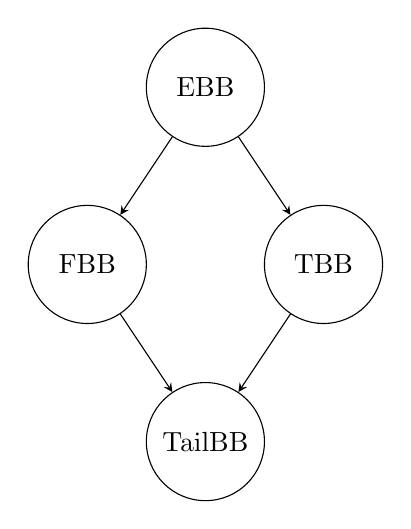
\begin{tikzpicture}[node distance=2cm and 3cm, >=stealth]
    % Style for consistent node dimensions
    \tikzstyle{node} = [circle, draw, fill=white, minimum size=1.5cm, inner sep=0]

    % Nodes
    \node[node] (EBB) at (1.5, 4.5) {EBB};
    \node[node] (TBB) at (3, 2.25) {TBB};
    \node[node] (FBB) at (0, 2.25) {FBB};
    \node[node] (TailBB) at (1.5, 0) {TailBB};

    % Edges
    \draw[->] (EBB) -- (TBB);
    \draw[->] (EBB) -- (FBB);
    \draw[->] (TBB) -- (TailBB);
    \draw[->] (FBB) -- (TailBB);
\end{tikzpicture}
\end{minipage}
    \caption{Code for \texttt{computeLoan} and the corresponding \textit{Diamond} Control Flow Graph.}
    \label{fig:calculate_loan}
\end{figure}

Considering the limitation of static analysis \cite{ritter2022anica}\cite{tan2024uncovering} and the nature of predication, the examples presented in this chapter are all highly computation-bounded rather than memory-bounded. As a consequence, the metrics that are going to be used to measure the performance of the various codes are \textit{IPC} and \textit{Total Execution Cycles} when executing the functions for 100 iterations.
It's worth mentioning that these are also the cases where predication tends to perform the best.

The first example presented in this section is the function \texttt{computeLoan}. This function and the corresponding Control Flow Graph are visible in Figure \ref{fig:calculate_loan}. This particular CFG shape is referred to as \textit{Diamond}.

When compiled with \texttt{-O0}, the resulting assembly code is visible in figure \ref{fig:calculate_loan_asm}, side by side with the corresponding \textit{if-converted} code.

\begin{figure}[H]
    \centering
    \begin{minipage}{0.45\textwidth}
    \begin{lstlisting}[style=AsmStyle]
computeLoan(bool, int):
    push    {r11, lr}
    mov     r11, sp
    sub     sp, sp, #16
    and     r0, r0, #1
    strb    r0, [r11, #-1]
    str     r1, [sp, #8]
    ldr     r0, [sp, #8]
    lsl     r0, r0, #1
    ldr     r1, .LCPI0_0
    bl      __aeabi_idiv
    str     r0, [sp, #4]
    ldrb    r0, [r11, #-1]
    tst     r0, #1
    beq     .LBB0_2
    ldr     r0, [sp, #8]
    ldr     r1, .LCPI0_3
    mul     r0, r0, r1
    ldr     r1, .LCPI0_0
    bl      __aeabi_idiv
    str     r0, [sp, #4]
    b       .LBB0_3
.LBB0_2:
    ldr     r0, [sp, #8]
    ldr     r1, .LCPI0_2
    mul     r0, r0, r1
    ldr     r1, .LCPI0_0
    bl      __aeabi_idiv
    str     r0, [sp, #4]
.LBB0_3:
    ldr     r0, [sp, #4]
    add     r0, r0, #5
    ldr     r1, .LCPI0_4
    bl      __aeabi_uidiv
    ldr     r1, .LCPI0_4
    mul     r0, r0, r1
    mov     sp, r11
    pop     {r11, pc}
    
.LCPI0_0:
    .long   100
.LCPI0_2:
    .long   7
.LCPI0_3:
    .long   5
.LCPI0_4:
    .long   10
    \end{lstlisting}
\end{minipage}%
\hspace{1cm}
\begin{minipage}{0.45\textwidth}
    \begin{lstlisting}[style=AsmStyle, numbers=right, belowskip=7.5\baselineskip]
computeLoan(bool, int):
    push    {r11, lr}
    mov     r11, sp
    sub     sp, sp, #16
    and     r0, r0, #1
    strb    r0, [r11, #-1]
    str     r1, [sp, #8]
    ldr     r0, [sp, #8]
    lsl     r0, r0, #1
    ldr     r1, .LCPI0_0
    bl      __aeabi_idiv
    str     r0, [sp, #4]
    ldrb    r0, [r11, #-1]
    ldr     r3, .LCPI0_3
    ldr     r4, .LCPI0_2
    @cmp     r0, #1
    @@mov     r1, r3
    @@movne   r1, r4
    ldr     r0, [sp, #8]
    mul     r0, r0, r1
    ldr     r1, .LCPI0_0
    bl      __aeabi_idiv
    str     r0, [sp, #4]
    ldr     r0, [sp, #4]
    add     r0, r0, #5
    ldr     r1, .LCPI0_4
    bl      __aeabi_uidiv
    ldr     r1, .LCPI0_4
    mul     r0, r0, r1
    mov     sp, r11
    pop     {r11, pc}

.LCPI0_0:
    .long   100
.LCPI0_2:
    .long   7
.LCPI0_3:
    .long   5
.LCPI0_4:
    .long   10    
    \end{lstlisting}
\end{minipage}%

    \caption[\texttt{ARMv7} Assembly Code of \textit{computeLoan}]{The \texttt{ARMv7} assembly code of \textit{computeLoan} when compiled using \texttt{-O0} code (on the left) and the \texttt{ARMv7} assembly code of \textit{computeLoan} when compiling using \textit{if-conversion} (on the right).}
    \label{fig:calculate_loan_asm}
\end{figure}

As in the \texttt{ARMv7} architecture predication plays a central role, predicated instructions are used on both sides of the assembly translation shown in figure \ref{fig:calculate_loan_asm}. On the left side, \texttt{tst}, \texttt{beq} and \texttt{b} implement the branch at the end of the \textit{EBB} block.
The instruction \texttt{tst} checks the least significant bit of \texttt{r0} (which contains the boolean value). The result of this test determines whether the branch will be taken or not by the instructions \texttt{beq}.

In the \textit{if-converted} code, the branches are totally removed, and the code becomes branchless. This is, as expected, done using predicated instructions. In particular, the region where this is done is highlighted on the right part of Figure \ref{fig:calculate_loan_asm}.
The instruction \texttt{cmp} is used to perform a comparison and set the special registers. The instruction \texttt{mov} will be executed in any case, but, \texttt{movne} will only be executed if the result of \texttt{cmp} is not equal. When this is the case, the changes made by \texttt{mov} will be overwritten.

The second example is the function \texttt{processOrder} which is displayed with the corresponding CFG in figure \ref{fig:processOrder}. This CFG shape takes the name of \textit{Forked Diamond}.

\begin{figure}[H]
    \centering
    \begin{minipage}{0.50\textwidth}
    \begin{lstlisting}[style=CStyle]
#include <cstdint>

enum class CustomerType { 
    REGULAR, PREMIUM 
};

uint32_t 
processOrder(CustomerType customerType,
             uint32_t orderAmount,
             uint32_t loyaltyPoints,
             uint32_t specialEvent) 
{
  if (customerType == 
        CustomerType::REGULAR) {
    if (orderAmount > 100) {
      return orderAmount - 10;
    } else {
      return orderAmount;
    }
  else
    if (loyaltyPoints > 500) {
      return orderAmount - 10;
    } else {
      ++loyaltyPoints;
      return orderAmount;
    }
  }
}
    \end{lstlisting}
\end{minipage}%
\hspace{-1cm} % Adjust horizontal overlap
\begin{minipage}{0.40\textwidth}
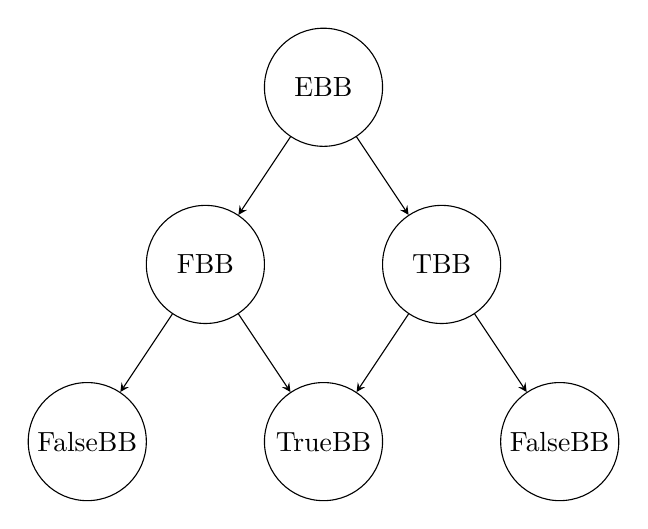
\begin{tikzpicture}[node distance=2cm and 3cm, >=stealth]
    % Style for consistent node dimensions
    \tikzstyle{node} = [circle, draw, fill=white, minimum size=1.5cm, inner sep=0]

    % Nodes
    \node[node] (EBB) at (1.5, 4.5) {EBB};
    \node[node] (TBB) at (3, 2.25) {TBB};
    \node[node] (FBB) at (0, 2.25) {FBB};
    \node[node] (TrueBB) at (1.5, 0) {TrueBB};
    \node[node] (FalseBB1) at (-1.5, 0) {FalseBB};
    \node[node] (FalseBB2) at (4.5, 0) {FalseBB};

    % Edges
    \draw[->] (EBB) -- (TBB);
    \draw[->] (EBB) -- (FBB);
    \draw[->] (TBB) -- (TrueBB);
    \draw[->] (TBB) -- (FalseBB2);
    \draw[->] (FBB) -- (TrueBB);
    \draw[->] (FBB) -- (FalseBB1);
\end{tikzpicture}
\end{minipage}
    \caption[Process Order Code and \textit{Forked Diamond}]{The C++ code for the function \texttt{processOrder}. The corresponding \textit{Forked Diamond} Control Flow Graph.}
    \label{fig:processOrder}
\end{figure}

\begin{figure}[H]
    \centering
    \begin{minipage}{0.45\textwidth}
    \begin{lstlisting}[style=AsmStyle]
    processOrder
        sub     sp, sp, #20
        str     r0, [sp, #12]
        str     r1, [sp, #8]
        str     r2, [sp, #4]
        str     r3, [sp]
        ldr     r0, [sp, #12]
        cmp     r0, #0
        bne     .LBB0_4
        ldr     r0, [sp, #8]
        cmp     r0, #100
        bls     .LBB0_3
        ldr     r0, [sp, #8]
        sub     r0, r0, #10
        str     r0, [sp, #16]
        b       .LBB0_7
    .LBB0_3:
        ldr     r0, [sp, #8]
        str     r0, [sp, #16]
        b       .LBB0_7
    .LBB0_4:
        ldr     r0, [sp, #4]
        cmp     r0, #500
        bls     .LBB0_6
        ldr     r0, [sp, #8]
        sub     r0, r0, #10
        str     r0, [sp, #16]
        b       .LBB0_7
    .LBB0_6:
        ldr     r0, [sp, #4]
        add     r0, r0, #1
        str     r0, [sp, #4]
        ldr     r0, [sp, #8]
        str     r0, [sp, #16]
    .LBB0_7:
        ldr     r0, [sp, #16]
        add     sp, sp, #20
        bx      lr
    \end{lstlisting}
\end{minipage}%
\hspace{1cm}
\begin{minipage}{0.45\textwidth}
    \begin{lstlisting}[style=AsmStyle, numbers=right, belowskip=14.5\baselineskip]
processOrder
    sub     sp, sp, #20
    str     r0, [sp, #12]
    str     r1, [sp, #8]
    str     r2, [sp, #4]
    str     r3, [sp]
    ldr     r0, [sp, #12]
    cmp     r0, #0
    @ldrne   r0, [sp, #4]
    @@addle   r0, r0, #1
    @@strle   r0, [sp, #4]
    ldr     r0, [sp, #8]
    cmp     r0, #100
    @@subhi   r0, r0, #10
    str     r0, [sp, #16]
    ldr     r0, [sp, #12]
    cmp     r0, #0
    @ldrne   r0, [sp, #4]
    @@cmpne   r0, #500
    @@subgt   r0, r0, #10
    @@strgt   r0, [sp, #16]
    ldr     r0, [sp, #16]
    add     sp, sp, #20
    bx      lr  
    \end{lstlisting}
\end{minipage}%
    \caption[\texttt{ARMv7} Assembly Code of \textit{processOrder}]{The \texttt{ARMv7} assembly code of \textit{processOrder} when compiled using \texttt{-O0} code (on the left) and the \texttt{ARMv7} assembly code of \textit{processOrder} when compiling using \textit{if-conversion} (on the right).}
    \label{fig:process_order_asm}
\end{figure}

In Figure \ref{fig:process_order_asm} it's possible to see the basic and the \textit{if-converted} versions of \texttt{processOrder}. The \textit{Forked Diamond CFG} enables more substantial code reduction if compared to the other \textit{if-conversion} seen so far. In this case, the number of predicated instructions is also much higher. For every three instructions in the \textit{if-converted} version, one is a predicated instruction.

\begin{figure}[H]
    \centering
    \centering
\begin{tikzpicture}
    \begin{axis}[
        width=10cm,
        height=7.5cm,
        ybar,
        symbolic x coords={ComputeLoan, ProcessOrder},
        xtick=data,
        ylabel={IPC (Percentage)},
        ymin=0, ymax=150,
        nodes near coords,
        bar width=25pt,
        axis lines=left,
        enlarge x limits=0.5,
        ytick={0,25,50,75,100,125,150},
        every axis label/.append style={font=\normalsize},
        every axis tick label/.append style={font=\small},
        legend style={at={(0.5,-0.15)}, anchor=north, legend columns=-1}, % Adjust legend position
        legend cell align={left}
    ]
        \addplot[pattern=dots, pattern color=red] coordinates {(ComputeLoan, 100) (ProcessOrder, 100)};
        \addlegendentry{Baseline}
        
        \addplot[pattern=north east lines, pattern color=red] coordinates {(ComputeLoan, 105.93) (ProcessOrder, 112.5)};
        \addlegendentry{Ifconverted}
    \end{axis}
\end{tikzpicture}
\hfill
\begin{tikzpicture}
    \begin{axis}[
        width=10cm,
        height=7.5cm,
        ybar,
        symbolic x coords={ComputeLoan, ProcessOrder},
        xtick=data,
        ylabel={Total Cycles (Percentage)},
        ymin=0, ymax=150,
        nodes near coords,
        bar width=25pt,
        axis lines=left,
        enlarge x limits=0.5,
        ytick={0,25,50,75,100,125,150},
        every axis label/.append style={font=\normalsize},
        every axis tick label/.append style={font=\small},
        legend style={at={(0.5,-0.15)}, anchor=north, legend columns=-1}, % Adjust legend position
        legend cell align={left}
    ]
        \addplot[pattern=dots, pattern color=blue] coordinates {(ComputeLoan, 100) (ProcessOrder, 100)};
        \addlegendentry{Baseline}
        
        \addplot[pattern=north east lines, pattern color=blue] coordinates {(ComputeLoan, 75.36) (ProcessOrder, 42.91)};
        \addlegendentry{Ifconverted}
    \end{axis}
\end{tikzpicture}

    \caption{Percentage variations of \textit{IPC} and \textit{Totaly Cycles} for the functions \texttt{computeLoan} (\textit{Diamon}) and \texttt{processOrder} (\textit{Forked Diamond}.)}
    \label{fig:benchmarks}
\end{figure}

The \textit{IPC} and \textit{total cycle} comparison of the two examples provided are showcased in figure \ref{fig:benchmarks}. From this, we can conclude that not only do the \textit{if-converted} versions have a higher \textit{IPC}, they are also shorter and therefore use a much lower number of \textit{Total Cycles}. 

The compiler heuristics mentioned in Section \ref{sec:compiler_heuristics} and the benchmarks reported in this section point out that whenever we face a \textit{CFG} with the shape of \textit{Diamond}, \textit{Forked Diamond} and \textit{Triangle}, applying \textit{if-conversion} results in improved performances.

\subsection{Compilers Limitations}
\label{sec:limitations}
In the examples reported in Section \ref{sec:predication_benchmark}, \textit{LLVM} always produced a great improvement when using \textit{if-conversion}. But, this is not always the case. Compilers are far from perfect, and it's not difficult to identify examples where a human ends up creating better code than a compiler.
The main reason for which performances are left on the table by compilers is because they fail to identify cases where \textit{if-conversion} could be applied.

An example of this can be crafted starting from the \texttt{computeLoan} example shown in Section \ref{sec:predication_benchmark}. As shown in the previous section, this is a perfect case to apply \textit{if-conversion} and this optimization results in a noticeable performance improvement.
Still, when the number of instructions and the complexity grows, compilers stop applying predication as the predicated block exceeds the size limit discussed in section \ref{sec:compiler_heuristics}. The new version of  \texttt{computeLoan} is referenced as \texttt{expandedComputeLoan} and is reported in Figure \ref{lst:expanded_compute_loan}, the performance measured for the \texttt{-O0} version is compared with a version where the \textit{if-conversion} optimization is applied manually. The corresponding assembly code is provided in appendix \ref{app:first}. From the figure, we can see that even though the compiler decided not to apply this optimization, applying still results in a great performance improvement as it is possible to see in Figure \ref{fig:compute_loan_ipc}.

\begin{figure}[h]
    \begin{lstlisting}[style=CStyle]
#include <cstdint>

uint32_t computeLoanPayment(bool isHouseLoan, uint32_t principal) 
{ 
    uint32_t baseRate = 0; 
@    uint32_t tax = principal * 2 / 100; 
    
    if (isHouseLoan) {
         baseRate = principal * 5 / 100; 
@@       baseRate += 50; 
    } else { 
        baseRate = principal * 7 / 100; 
@@      baseRate += 30; 
    } 
    
@@    uint32_t totalPayment = baseRate + tax; 
@@    totalPayment = (totalPayment + 5) / 10 * 10; 
    return totalPayment; 
}
\end{lstlisting}

    \caption{The expanded \texttt{computeLoan} function. The added lines are highlighted in red.}
    \label{lst:expanded_compute_loan}
\end{figure}

\begin{figure}[h]
    \begin{minipage}{0.42\textwidth}
    \centering
        \begin{tikzpicture}
            \begin{axis}[
                width=5.5cm,
                height=7.5cm,
                ybar,
                symbolic x coords={Baseline, If-converted},
                xtick=data,
                ylabel={IPC (Percentage)},
                ymin=0, ymax=150,
                nodes near coords,
                bar width=25pt,
                axis lines=left,
                enlarge x limits=0.5,
                ytick={0,25,50,75,100,125,150},
                every axis label/.append style={font=\normalsize},
                every axis tick label/.append style={font=\small}
            ]
                \addplot[pattern=north east lines, pattern color=red] coordinates {(Baseline, 100) (If-converted, 118.18)};
            \end{axis}
        \end{tikzpicture}
\end{minipage}
\hfill
\begin{minipage}{0.42\textwidth}
    \centering
    \begin{tikzpicture}
        \begin{axis}[
            width=5.5cm,
            height=7.5cm,
            ybar,
            symbolic x coords={Baseline, If-converted},
            xtick=data,
            ylabel={Total Cycles (Percentage)},
            ymin=0, ymax=150,
            nodes near coords,
            bar width=25pt,
            axis lines=left,
            enlarge x limits=0.5,
            ytick={0,25,50,75,100,125,150},
            every axis label/.append style={font=\normalsize},
            every axis tick label/.append style={font=\small}
        ]
            \addplot[pattern=north east lines, pattern color=blue] coordinates {(Baseline, 100) (If-converted, 51.29)};
        \end{axis}
    \end{tikzpicture}
\end{minipage}

    \caption{\textit{IPC} and \textit{Total Cycles} reported for \texttt{expandedComputeLoan} by \textit{LLVM-MCA}.}
    \label{fig:compute_loan_ipc}
\end{figure}

The heuristics used by the compilers, and described in section \ref{sec:compiler_heuristics}, are designed to be general and provide good results in most scenarios, the compiler's knowledge at compile time is inherently limited, and applying more complex optimization would require more compilation time.

\newpage